%todo bilder in tabelle ausrichten
\chapter{Features}\label{Features}
Dieses Kapitel beschreibt die Bedienung und die Möglichkeiten des Programms.
\begin{figure}[htbp]
\centering
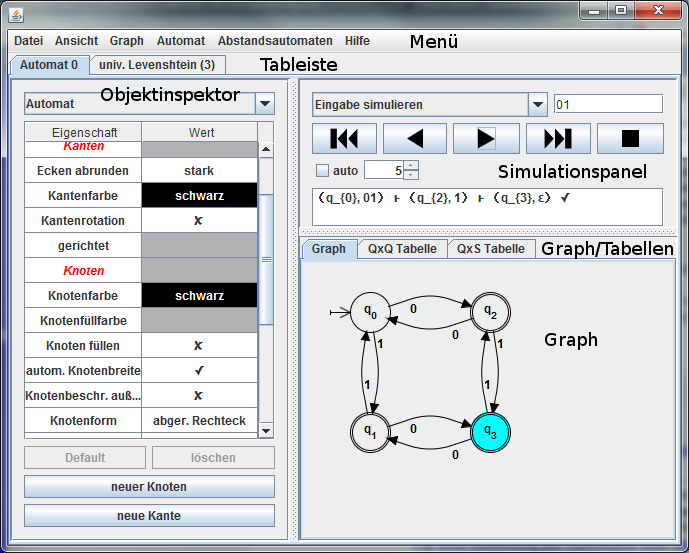
\includegraphics[width=\linewidth,height=\textheight,keepaspectratio]{pic/screenshots/all-text}%
\caption{Übersicht über das Programm}%
\end{figure}
\section{Allgemeines}
Das Programm dient in erster Linie dazu, Automaten zu konstruieren und simulieren. Da bei der Automatenkonstruktion und -darstellung eine Konstruktion und Darstellung für allgemeine Graphen enthalten ist, gibt es auch die Möglichkeit, Graphen ohne Automateneigenschaften zu erstellen. Diese können nicht simuliert werden, haben keine $Q \times S$-Tabellendarstellung und keine Übergangsfunktion. Dafür können für Kanten Gewichte eingestellt werden und es können ungerichtete Kanten benutzt werden.

Es können beliebig viele Graphen und Automaten geöffnet werden, welche dann in der Tableiste auswählbar sind.
Über das \textit{Datei}-Menü können neue Graphen oder Automaten erstellt werden.\\
Automaten und Graphen können gespeichert und geladen werden. Außerdem wird eine Liste zuletzt benutzter Dateien angezeigt, mit deren Hilfe Dateien schneller geladen werden können.\\
Bilder von Graphen können im PNG-Format exportiert werden. Dabei wird nicht der sichtbare Bereich, sondern der vollständige Graph ohne Ränder exportiert. Der Hintergrund ist transparent.\\
Im Menü \textit{Ansicht} kann das Java-Look'n'Feel geändert werden.\\
Das Menü \textit{Hilfe} beinhaltet eine Übersicht zur Steuerung des Graphen und Informationen zum Programm.

Namen und Kommentare können tief- und hochgestellte Teile enthalten. Dabei wird die in \LaTeX \ übliche Formatierung benutzt, also \_ zum Tiefstellen und \^\  zum Hochstellen. Geschweifte Klammern dienen zur Blockbildung, ohne Block gilt das Formatierungszeichen nur für das nachfolgende Zeichen. Mit Backslashes kann die Funktion des Formatierungszeichens deaktiviert werden (Escapen). Um ein Backslash vor einem solchen Zeichen anzuzeigen, sind zwei Backslashes nötig.
\begin{figure}[!htbp]
\centering
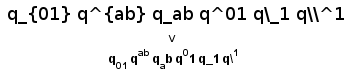
\includegraphics[scale=0.7]{pic/parseString}%
\caption{Beispiel für die Umsetzung von Hoch- und Tiefstellung}%
\end{figure}
\section{Automaten}
Die Automaten unterliegen keinen besonderen Einschränkungen. Ein Alphabet wird nicht vorgegeben, es ergibt sich automatisch aus den benutzten Übergangslabeln. Es dürfen beliebig viele Start- und Endzustände definiert werden. Es ist ebenfalls möglich, mehrere Kanten mit gleichen Start- und Zielknoten zu machen, was aber gleichwertig zu einer Kante mit mehreren Übergangslabeln ist. Kanten können optional mit einem Namen versehen werden. Knoten werden automatisch durchnummeriert (q$_n$ bzw. v$_n$), dieser Name kann aber nach Belieben geändert werden. Mehrere Knoten mit gleichem Namen sind möglich, aber nicht empfehlenswert.

Die Simulation unterstützt Nichtdeterminismus, spontane Übergänge, Any-Über\-gänge (alle Symbole treten als Übergang auf), Else-Über\-gänge (alle Symbole, außer denen, für die ein expliziter Übergang definiert ist, treten als Übergang auf), Übergangslabel variabler Länge (Blöcke) und Symbolabkürzungen, wobei einzelne Zeichen gegen verschiedene andere Zeichen ersetzt werden können. Für Details bezüglich der Sonderzeichen siehe entsprechende Einträge bei den Automateneigenschaften im Abschnitt über den Objektinspektor.

%Determinismus
\label{Determinismus}
Die Sonderfunktionen für die Simulation machen es sinnvoll, sich Gedanken über den Determinismusbegriff zu machen. Es ist klar, dass ein Automat mit mehreren Startzuständen nichtdeterministisch ist. Ein Automat wird ebenfalls nichtdeterministisch, wenn es von einem Zustand aus neben einem Any-Übergang noch Übergänge zu anderen Zuständen außer Else-Übergängen gibt. Else-Übergänge beeinflussen den Determinismus nur, wenn es von einem Zustand mehrere Else-Übergänge zu unterschiedlichen Zielzuständen gibt.\\
Spontane Übergänge bringen einen gewissen Nichtdeterminismus mit, weil ggf. in einem Schritt entschieden werden muss, ob ein normaler Übergang oder ein spontaner Übergang erfolgen soll. Man kann aber einen Determinismus definieren, dass es eindeutig sein muss, ob für eine erfolgreiche Weiterverarbeitung der Eingabe ein spontaner Übergang erfolgen muss oder nicht darf. Das bedeutet, es darf nur von maximal einem Epsilon-erreichbarkeien Zustand ein Übergang mit einem Symbol x möglich sein. Das erfordert einen Lookahead. Diese Definition von Determinismus soll hier gelten.\\
Lässt man nur Blöcke fester Länge n zu, braucht man für Determinismus keine besonderen Einschränkungen. Eine mögliche Interpretation wäre, den Block nicht als $n$ konkatenierte Symbole aus dem Alphabet $S$, sondern als ein Symbol der Länge $n$ aus dem Alphabet $S^n$ zu betrachten. Problematisch wird es bei Blöcken variabler Länge. Wenn man als einzige Forderung stellt, dass die Übergangsrelation eine Funktion ist, wäre es möglich, dass von einem Zustand zwei Übergänge existieren, wobei der eine Übergang ein echtes Präfix des anderen ist und trotzdem jede Berechnung eindeutig ist. Diese Eindeutigkeit ist schwer feststellbar. Daher soll hier die restriktivere Variante gelten, dass in einem Zustand kein Übergang Präfix eines anderen sein darf (siehe auch Beispiele). Die spontanen Übergänge, die echtes Präfix eines jeden nicht spontanen Überganges sind, bilden hier eine Ausnahme.
\begin{figure}[!htbp]
\centering
\subfloat[NEA: Mayaren führt von q$_0$ zu q$_2$ und q$_4$ -- deshalb Forderung der Präfixeigenschaft]{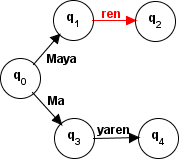
\includegraphics[scale=0.7]{pic/automata/bspMayarenndet}}%
%\hfill
\hspace{0.1cm}
\subfloat[DEA-Version von (a): die Übergänge wurden nach Präfix zerlegt.]{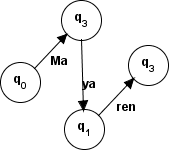
\includegraphics[scale=0.7]{pic/automata/bspMayarendet}}%
%\\
\hspace{0.1cm}
\subfloat[NEA wegen verletzter Präfixeigenschaft, obwohl für jede Eingabe die Berechnung eindeutig ist.]{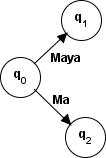
\includegraphics[scale=0.7]{pic/automata/bspMayandet}}%
%\hfill
\hspace{0.1cm}
\subfloat[DEA: dass beide Übergänge das Präfix \glqq Ma\grqq haben, spielt keine Rolle.]{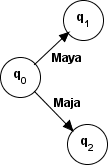
\includegraphics[scale=0.7]{pic/automata/bspMayadet}}%
\caption{Beispiele Determinismus}%
\end{figure}

%Menü Automat
Im Menü \textit{Automat} finden sich einige Algorithmen. Unter \textit{Elimination spontaner Übergänge} können spontane Übergänge von links, von rechts oder beidseitig durch Absorbtion von normalen Übergängen eliminiert werden.\\
Im Submenü \textit{Minimierung} können unerreichbare Zustände, unproduktive Zustände und unnötige Kanten entfernt werden. \textit{Unnötige Kanten entfernen} bedeutet, dass Mehrfachkanten mit gleichem Start- und Zielknoten zusammengefasst werden und Kanten ohne Übergänge entfernt werden. Minimierungsalgorithmen für DEAs oder gar NEAs sind noch nicht implementiert.\\
Die Potenzmengenkonstruktion macht aus einem NEA einen gleichwertigen DEA. Dies liefert einen neuen Automaten, der ursprüngliche Automat bleibt also erhalten.\\
Transformation in den dualen Automaten bedeutet das Austauschen von Start- und Zielzuständen und die Umkehrung aller Kanten.\\
\textit{Hotel Calfornia Zustand hinzufügen} fügt dem Automaten einen Zustand hinzu, der nicht zur erkannten Sprache beiträgt, aber den Automaten vollständig macht; es führen also alle nicht definierten Übergänge in diesen Zustand.\\
Der Kleene-Algorithmus zur Identifikation der Sprache durch einen regulären Ausdruck ist noch nicht implementiert.\\
\textit{Automat untersuchen} zeigt ein Fenster, in dem steht, ob der Automat vollständig ist oder nicht (also ob es von jedem Zustand mit jedem Symbol des Alphabetes einen Übergang gibt), ob es sich um einen NEA oder DEA handelt und ob der Automat spontane Übergänge benutzt. Außerdem werden alle Zustände aufgelistet und deren Anzahl angegeben. Es wird das minimale Alphabet bestimmt und Start- und Endzustandsmenge angezeigt.

%Menü Abstandsautomaten
Im Menü \textit{Abstandsautomaten} sind Funktionen zur Konstruktion spezieller und universeller Abstandsautomaten zu finden. Außerdem kann hier das Tool zur Kodierung der Eingabe für universelle Abstandsautomaten aufgerufen werden. Zur Funktionsweise der Automaten siehe Kapitel \ref{Abstandsautomaten} über Abstandsautomaten.
\section{Objektinspektor}
\begin{figure}[!htbp]
\centering
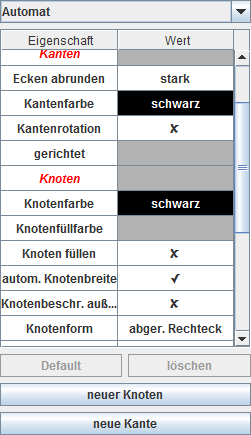
\includegraphics{pic/screenshots/oi}%
\caption{Der Objektinspektor}%
\end{figure}
Der Objektinspektor ist die Leiste bzw. Tabelle am linken Fensterrand und dient dazu – je nach  Auswahl – Eigenschaften vom Graphen bzw. Automaten, Knoten bzw. Zustand oder Kante bzw. Übergang zu ändern. Über der Tabelle ist eine ComboBox zur Auswahl des gewünschten Elementes. Unter der Tabelle sind Buttons zum Hinzufügen von Knoten und Kanten und zum Löschen und Zurücksetzen der Standardeinstellungen für Kanten und Knoten.
\subsection{Graph bzw. Automat}
\begin{figure}[!htbp]
\centering
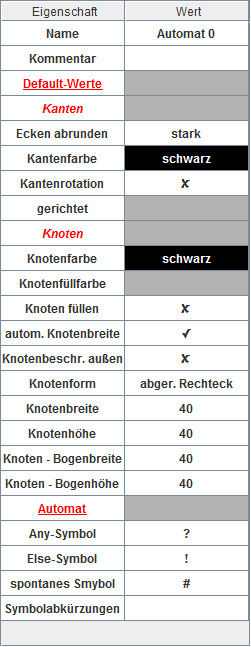
\includegraphics[scale=0.8]{pic/screenshots/oi-automat}%
\caption{Die Automatenansicht des Objektinspektors}%
\end{figure}
%\begin{table}
\begin{oitable}
Name&
Der Name hat keine besondere Bedeutung. Er wird beim Speichern vorgeschlagen und nach dem Laden als Bezeichnung des Tabs angezeigt.&
Automat n,\newline Graph n\\
\hline
Kommentar&
Im Kommentar kann z.B. die Funktion des Graphen bzw. Automaten beschrieben werden. Diese wird dann, wenn der Graph ausgewählt ist, oben in der graphischen Ansicht angezeigt.&
\\
\hline
Default-Werte&
Für die Beschreibung der Default-Werte für Knoten und Kanten, siehe entsprechende Werte in den Unterkapiteln.&\\
\end{oitable}
%\caption{Eigenschaften von Graphen ohne Default-Werte}
%\end{table}

Automaten haben noch einige zusätzliche Eigenschaften.

%\begin{table}
\begin{oitable}
Any-Symbol&
Das Any-Symbol steht für einen beliebigen Übergang. Dieser Übergang kann für jedes beliebige Zeichen der Eingabe benutzt werden. Zu beachten ist, dass es nur für ein einzelnes Symbol steht und nicht in Blöcken benutzt werden kann.&?\\
\hline
Else-Symbol&
Das Else-Symbol kann genau dann als Übergang benutzt werden, wenn es für das aktuelle Zeichen der Eingabe keinen anderen möglichen Übergang gibt. Es ist ähnlich wie das Any-Symbol, jedoch bleibt Determinismus erhalten. Zu Beachten: Spontane Übergänge beeinflussen Else-Übergänge nicht. Gibt es mehrere Else-Übergänge sind alle gleichwertig. Gibt es für jedes Zeichen einen anderen Übergang (z.B. durch ein Any-Übergang), ist der Else-Übergang leer.&!\\
\hline
Spontanes Symbol&
Das spontane Symbol (typischerweise ein $\epsilon$ - aufgrund der einfacheren Eingabe per Default ein \#) ist ein Übergang, der benutzt werden kann ohne ein Zeichen der Eingabe zu verbrauchen. Es können mehrere spontane Übergänge hintereinander ausgeführt werden.&\#\\
\hline
Symbol\-abkürzungen&
Symbolabkürzungen sind eine Menge von Abbildungen eines einzelnes Zeichens auf eine Menge von Zeichen. Hier kann z.B. definiert werden, dass ein \glqq\_\grqq für eine 0 oder eine 1 stehen kann. Gibt es bei der Simulation einen Übergang \_ kann dieser bei einer 0 oder einer 1 in der Eingabe benutzt werden. Symbolabkürzungen können auch in Blöcken benutzt werden. (Aber es können nicht einzelne Symbole auf Symbolblöcke abgebildet werden.)
\end{oitable}
%\caption{Besondere Eigenschaften von Automaten}
%\end{table}
\subsection{Knoten}
\begin{figure}[!htbp]
\centering
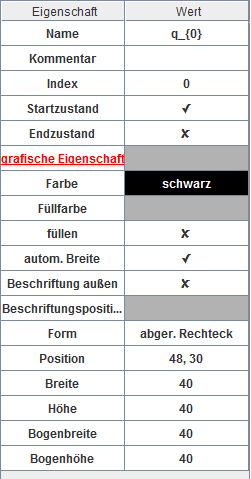
\includegraphics[scale=0.8]{pic/screenshots/oi-knoten}%
\caption{Die Knotenansicht des Objektinspektors}%
\end{figure}
%\begin{table}
\begin{oitable}
Name&
Der Name ist die Bezeichnung und Beschriftung des Knotens. Außerdem werden Knoten in Listen durch diesen Namen angezeigt.&
$q_n$ für Automaten, $v_n$ für Graphen\\
\hline
Kommentar&
Bei Auswahl des Knotens, wird der Kommentar oben in der grafischen Ansicht angezeigt. Dieser kann z.B. eine Beschreibung der Bedeutung des Knotens enthalten.&\\
\hline
Index&
Der Index ist wichtig bei der Simulation der Konstruktion. Dabei wird schrittweise der Index erhöht und jeweils nur Knoten und Kanten angezeigt, deren Index kleiner oder gleich dem aktuellen Index ist.&0\\
\hline
Startzustand&
Ist dieser Zustand Startzustand? Dies sind Zustände, in denen die Simulation einer Eingabe beginnen kann. Grafische Darstellung: ein eingehender Pfeil am linken Rand. In der Tabelle in der Zeile/Spalte I (für Initial) aufgefürt.&
\includegraphicstotab[scale=0.7]{pic/einstellungen/knoten-start}\\
\hline
Endzustand&
Ist dieser Zustand Endzustand? Endet die Simulation einer Eingabe in einem Endzustand, wird die Eingabe akzeptiert. Grafische Darstellung: Zustand ist doppelt umrandet. In der Tabelle in der Zeile/Spalte F (für Final) aufgeführt. &
\includegraphicstotab[scale=0.7]{pic/einstellungen/knoten-ziel}\\
\end{oitable}
%\caption{Funktionale Eigenschaften der Knoten}
%\end{table}
Grafische Eigenschaften
%\begin{table}
\begin{oitable}
Farbe&
Die Farbe der Umrandung und Beschriftung.&
\includegraphicstotab[scale=0.7]{pic/einstellungen/knoten-farbe}\\
\hline
Füllfarbe&
Die Farbe, in der der Knoten gefüllt wird. Nur auswählbar, wenn Füllen aktiviert ist.&
\includegraphicstotab[scale=0.7]{pic/einstellungen/knoten-fuellung}\\
\hline
Füllen&
Wenn nicht aktiviert, ist der Knoten nicht gefüllt, sonst mit der unter Füllfarbe festgelegten Farbe.&\\
\hline
Automatische Breite&
Wenn aktiviert, wird der Knoten automatisch verbreitert, wenn die Beschriftung breiter als der Knoten ist.&
\includegraphicstotab[scale=0.7]{pic/einstellungen/knoten-beschr-a} \includegraphicstotab[scale=0.7]{pic/einstellungen/knoten-beschr-b}\\
\hline
Beschriftung außen&
Soll die Beschriftung des Knotens frei außerhalb des Knotens platzierbar sein. Wenn nicht aktiviert, ist die Beschriftung immer an der gleichen Stelle und genauso groß wie der Knoten.&
\includegraphicstotab[scale=0.7]{pic/einstellungen/knoten-aussen}\\
\hline
Beschriftungs\-position&
Die Position der Beschriftung in Pixeln. Nur auswählbar, wenn \textit{Beschriftung außen} aktiviert ist.&\\
\hline
Form&
Form des Knotens: abgerundetes Rechteck, Ellipse oder Rechteck. Bemerkung: Kreis und Quadrat sind Spezialfälle von Ellipse und Rechteck (oder auch vom abgerundeten Rechteck).&
\includegraphicstotab[scale=0.7]{pic/einstellungen/knoten-form-a} \includegraphicstotab[scale=0.7]{pic/einstellungen/knoten-form-b} \includegraphicstotab[scale=0.7]{pic/einstellungen/knoten-form-c}\\
\hline
Position&
Die Position des Knotens in Pixeln.&\\
\hline
Breite&
Breite des Knotens in Pixeln.&40\\
\hline
Höhe&
Höhe des Knotens in Pixeln.&40\\
\hline
Bogenbreite&
Nur für abgerundetes Rechteck: Wie viele Pixel in x-Richtung werden abgerundet.&40\\
\hline
Bogenhöhe&
Nur für abgerundetes Rechteck: Wie viele Pixel in y-Richtung werden abgerundet.&40\\
\end{oitable}
%\caption{Grafische Eigenschaften von Knoten}
%\end{table}
\subsection{Kanten}
\begin{figure}[!htbp]
\centering
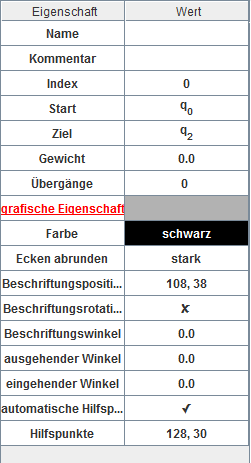
\includegraphics[scale=0.8]{pic/screenshots/oi-kanten}%
\caption{Die Kantenansicht des Objektinspektors}%
\end{figure}
%\begin{table}
\begin{oitable}
Name&
Der Name wird der Kantenbeschriftung vorangestellt.&\\
\hline
Kommentar&
Bei Auswahl des Knotens, wird der Kommentar oben in der grafischen Ansicht angezeigt. Dieser kann z.B. eine Beschreibung der Bedeutung der Kante enthalten.&\\
\hline
Index&
Der Index ist wichtig bei der Simulation der Konstruktion. Dabei wird schrittweise der Index erhöht und jeweils nur Knoten und Kanten angezeigt, deren Index kleiner oder gleich dem aktuellen Index ist.&0\\
\hline
Start&
Der Zustand, von dem die Kante losgeht.&\\
\hline
Ziel&
Der Zustand, zu dem die Kante hingeht.&\\
\hline
Gewicht&
In der Graphentheorie haben gewichtete Kanten Bedeutung. Für Graphen wird das Kantengewicht (sofern nicht NaN) neben dem Namen der Kante als Beschriftung angezeigt. Für Automaten hat das Kantengewicht keine Bedeutung und wird nicht angezeigt.&none\\
\hline
gerichtet&
Nur einstellbar für Graphen. Ist die Kante gerichtet (mit Pfeil) oder nicht. Kanten von Automaten sind immer gerichtet.&true\\
\hline
Übergänge&
Nur für Automaten. Mit welchen Symbolen bzw. Symbolblöcken kann diese Kante als Übergang in den Zielzustand benutzt werden.&\\
\end{oitable}
%\caption{Funktionale Eigenschaften von Kanten}
%\end{table}
Grafische Eigenschaften
%\begin{table}
\begin{oitable}
Farbe&
Die Farbe der Kante und der Beschriftung.&
\includegraphicstotab[scale=0.7]{pic/einstellungen/kanten-farbe}\\
\hline
Ecken abrunden&
Durch Hilfspunkte können Ecken/Kurven in Kanten eingebaut werden. Ob diese Ecken abgerundet werden oder nicht kann hier ausgewählt werden. Für nähere Informationen siehe entsprechendes Kapitel in der Implementierung.&
\includegraphicstotab[scale=0.7]{pic/einstellungen/kanten-abrundung-a} \includegraphicstotab[scale=0.7]{pic/einstellungen/kanten-abrundung-b} \includegraphicstotab[scale=0.7]{pic/einstellungen/kanten-abrundung-c}\\
\hline
Beschriftungs\-position&
Die Position in Pixeln, an der die Beschriftung ist. Bei Neuberechnung der Kante wird die Position neu berechnet (und muss ggf. erneut angepasst werden).&\\
\hline
Beschriftungs\-rotation&
Wenn aktiviert, wird die Beschriftung am Beginn der Kante positioniert und in dem ausgehenden Winkel der Kante gedreht.\newline
Wenn deaktiviert, wird die Beschriftung horizontal in der Mitte zwischen Start und erstem Hilfspunkt (bzw. Ziel) positioniert.&\includegraphicstotab[scale=0.7]{pic/einstellungen/kanten-beschriftungrot-a} \includegraphicstotab[scale=0.7]{pic/einstellungen/kanten-beschriftungrot-b}\\
\hline
Beschriftungs\-winkel&
Bei Neuberechnung der Kante wird der Winkel neu berechnet (und muss ggf. erneut angepasst werden).&\\
\hline
ausgehender Winkel&
Sofern nicht anders festgelegt, wird der ausgehende Winkel automatisch berechnet. Hiermit kann festgelegt werden, an welcher Stelle des Knotens die Kante verankert ist. Hinweis: Die Kante tritt nicht orthogonal aus dem Knoten, dies kann durch zusätzliche Hilfspunkte erreicht werden (der ausgehende Winkel allerdings auch). 0° ist am rechten Rand und vertikal in der Mitte des Knotens.&\includegraphicstotab[scale=0.7]{pic/einstellungen/kanten-deg}\\
\hline
eingehender Winkel&
Sofern nicht anders festgelegt, wird der eingehende Winkel automatisch berechnet. Hiermit kann festgelegt werden, an welcher Stelle des Knotens die Kante verankert ist. Hinweis: Die Kante tritt nicht orthogonal in den Knoten, dies kann durch zusätzliche Hilfspunkte erreicht werden (der ausgehende Winkel allerdings auch). 0° ist am rechten Rand und vertikal in der Mitte des Knotens.&
\includegraphicstotab[scale=0.7]{pic/einstellungen/kanten-deg}\\
\hline
automatische Hilfspunkte&
Wenn aktiviert, werden für Schleifen und direkten Hin- und Rückkanten automatisch Hilfspunkte angelegt, sodass eine Schleife als solche erkennbar ist und die Kanten nicht übereinander liegen. Wenn der Menüpunkt rechtwinklige Kanten im Menü Graph aktiviert ist, werden Hilfspunkte derart angelegt, dass Kanten nur vertikal und horizontal verlaufen. Die Hilfspunkte werden bei jeder Neuberechnung der Kante neu angelegt und ggf. vorhandene Hilfspunkte werden gelöscht. Werden die Hilfspunkte verändert, wird dies automatisch deaktiviert.&
\includegraphicstotab[scale=0.7]{pic/einstellungen/kanten-autosp-a} \includegraphicstotab[scale=0.7]{pic/einstellungen/kanten-autosp-b} \includegraphicstotab[scale=0.7]{pic/einstellungen/kanten-autosp-c}\\
\hline
Hilfspunkte&
Eine Liste von Punkten, an denen die Kante entlanggeleitet wird.&
\includegraphicstotab[scale=0.7]{pic/einstellungen/kanten-sp}\\
\end{oitable}
%\caption{Grafische Eigenschaften von Kanten}
%\end{table}
\section{Graphische Ansicht}
\begin{figure}[!htbp]
\centering
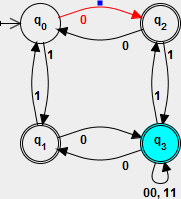
\includegraphics{pic/screenshots/graph}%
\caption{Die graphische Ansicht}%
\end{figure}
Die graphische Ansicht ist die Hauptansicht für Graphen und Automaten. Automaten werden hier mit Knoten für Zustände und Kanten für Übergänge dargestellt.

Über den Menüpunkt \textit{Graph am Raster ausrichten} im Menü \textit{Graph} können die Knoten so positioniert werden, dass nur an diskreten Stellen Knoten sind. Dabei wird auch beachtet, dass keine Knoten übereinander liegen. Dabei werden die Knoten der Reihe nach an den nächst besten freien Platz positioniert und in keiner Weise intelligent angeordnet.\\
Der Menüpunkt \textit{Spring Embedder} ist experimentell. Hierbei sollen die Knoten sinnvoll angeordnet werden, sodass verbundene Knoten beieinander liegen und zwischen Knoten ein gewisser Abstand ist. Das funktioniert bisher nur teilweise.\\
Mit dem Menüpunkt \textit{rechtwinklige Kanten} lässt sich einstellen, ob automatisch Hilfspunkte angelegt werden sollen, damit Kanten nur horizontal und vertikal verlaufen können.

Alle wichtigen Konstruktionsaufgaben und Einstellungsmöglichkeiten können mit Hilfe von Tastatur- und Mauseingaben direkt in dem Graphen vollzogen werden. Die folgende Übersicht zur Steuerung kann auch über den Punkt \textit{Bedienung Graph} im Menü \textit{Hilfe} angezeigt werden. Grundgedanke der Steuerung ist Linksklick zum Ziehen, Rechtsklick/Doppelklick zum Ertellen, Links Drag zum Verschieben und Mittelklick für andere Aufgaben.\\
\textit{Hinweis: Drag bedeutet klicken, nicht los lassen und ziehen}
\begin{itemize}                
\item Zustände
\begin{itemize}                
\item auswählen: Linksklick
\item neu: Rechtsklick oder Doppelklick mit links ins Leere
\item löschen: Auswählen, Entf drücken
\item verschieben: Links Drag
\item Start-/Endzustand durchschalten: Mittelklick
\item beschriften: Auswählen, Tastatureingabe (Backspace/Rücktaste zum Lö\-schen)
\end{itemize}
\item Kanten
\begin{itemize}                
\item auswählen: Linksklick
\item neu: Startknoten auswählen, Rechtsklick oder Doppelklick mit links auf den Zielknoten
\item löschen: Auswählen, Entf drücken
\item Ziel ändern: Auswählen, Rechtsklick oder Doppelklick mit links auf neuen Zielknoten
\item Übergang/Beschriftung ändern: Auswählen, Tastatureingabe (Back\-space/""Rück\-tas\-te zum Löschen)
\item Beschriftung verschieben: Links Drag auf Beschriftung
\item Beschriftungsrotation (de)aktivieren: Mittelklick auf Beschriftung
\item Hilfspunkte
\begin{itemize}                
\item neu: Links Drag an gewünschter Stelle
\item löschen: Kante auswählen, Mittelklick auf Hilfspunkt
\item verschieben: Links Drag auf Hilfspunkt
\item Abrundung der Ecken: Mittelklick auf die Kante (gar nicht, leicht, stark)
\end{itemize}
\end{itemize}
\item sonstiges
\begin{itemize}                
\item neue Kante mit Knoten: Rechts Drag vom Startknoten zum Zielknoten; existiert am Ziel keiner, wird er erstellt.
\item nichts auswählen: Linksklick ins Leere
\item alles verschieben: Rechts Drag im Leeren
\end{itemize}
\end{itemize}
\section{Tabellarische Ansicht}
\begin{figure}
\centering
%\hfill %
\subfloat[$Q \times Q$ \label{pic:qxq}]{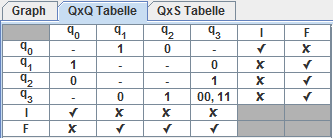
\includegraphics{pic/screenshots/tableqxq}}
\\%\hfill \\\hfill% alternativ auch \hspace{1cm} für genaue Angaben
\subfloat[$Q \times S$ \label{pic:qxs}]{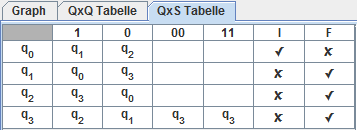
\includegraphics{pic/screenshots/tableqxs}}
%\hfill %
\caption{Tabellarische Ansichten zu dem obigen Graphen: a) $Q \times Q$, b) $Q \times S$ }
\label{table}
\end{figure}
Die Übergangsrelation von Automaten lässt sich als Teilmenge von $Q \times Q \times S$ auffassen. Da das kartesische Produkt kommutativ ist, lässt dies mehrere Darstellungen von Tabellen zu. Für Automaten sind, $Q \times Q$, wobei in den Zellen Symbole aus $S$ stehen und $Q \times S$, wobei in den Zellen die Zielzustände aus $Q$ stehen. Für Graphen gibt es nur die $Q \times Q$-Darstellung, wobei der Inhalt der Zellen zeigt, ob eine Kante von dem Startzustand (Zeile) zum entsprechenden Zielzustand (Spalte) existiert.

Bei $Q \times Q$ sind in Zeilen und Spalten die Zustände bzw. Knoten angeordnet. An den Kreuzungspunkten stehen die Kante mit den Übergängen, sofern eine existiert. Zwei zusätzliche Zeilen und Spalten zeigen an, ob der Zustand Startzustand (I) oder Endzustand (F) ist.\\
Durch Klick auf einen Zustand kann der Name des Zustandes geändert werden. Durch Klicks auf Startzustand- bzw. Endzustand-Felder kann der entsprechende Status gewechselt werden. Die Kanten werden textuell bearbeitet, wobei die einzelnen Übergänge durch \glqq , \grqq getrennt werden müssen. Ein Name kann vorangestellt werden, abgetrennt durch \glqq : \grqq . Zustände bzw. Knoten sollten durch den Button unter dem Objektinspektor hinzugefügt werden.

Bei $Q \times S$ sind in Zeilen die Zustände angeordnet und in den Spalten alle vorkommenden Übergänge. An den Kreuzungspunkten steht eine Liste von Zuständen, die vom entsprechenden Zustand mit dem entsprechendem Übergang erreichbar sind. Zwei zusätzliche Spalten zeigen an, ob der Zustand Startzustand (I) oder Endzustand (F) ist.\\
Durch Klick auf einen Zustand, kann der Name des Zustandes geändert werden. Durch Klicks auf Startzustand- bzw. Endzustand-Felder kann der entsprechende Status gewechselt werden. Die erreichbaren Zustände werden duch den Collection\-Editor bearbeitet, in dem Zustände hinzugefügt, gelöscht oder ausgetauscht werden können. Übergänge können mit dem Eingabefeld und den Buttons unter der Tabelle hinzugefügt oder entfernt werden. Zustände bzw. Knoten sollten durch den Button unter dem Objektinspektor hinzugefügt werden.

\textit{Für die Tabellen sollte noch eine Darstellung der Simulation folgen und eine Änderung der Auswahl.}
\section{Simulationspanel}
\begin{figure}[htbp]
\centering
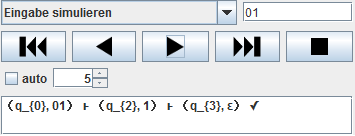
\includegraphics{pic/screenshots/simpanel}%
\caption{Das Simulationspanel - Bis auf das Feld oben rechts ist die Ansicht für Konstruktion und Berechnung genauso.}%
\end{figure}
Das Simulationspanel gibt es nur für Automaten.

\textit{Hinweis: Die Simulation funktioniert bisher nur mit der graphischen Ansicht.}

Das Simulationspanel kann genutzt werden um die Konstruktion, eine Eingabe oder eine spezielle Berechnung zu simulieren. Die Aufgabe kann mit der ComboBox oben links ausgewählt werden.

Mit 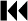
\includegraphics[height=1em]{pic/icons/beginning} kann die Simulation gestartet bzw. zurück auf den Anfang gesetzt werden. Mit 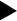
\includegraphics[height=1em]{pic/icons/next} und 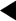
\includegraphics[height=1em]{pic/icons/last} kann schrittweise vor und zurück gegangen werden. 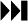
\includegraphics[height=1em]{pic/icons/end} beendet die Simulation, geht also zum letzten Schritt. 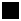
\includegraphics[height=1em]{pic/icons/stop} bricht die Simulation ab.\\
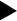
\includegraphics[height=1em]{pic/icons/next} ist so eingerichtet, dass es bei Bedarf fragt, ob die Simulation gestartet werden soll, wenn die Simulation noch nicht gestartet wurde. Wenn die CheckBox \textit{auto} aktiviert ist, folgt der nächste Schritt automatisch nach der im Spinner festgelegten Anzahl von Sekunden.
\subsection{Konstruktion}
Bei der Simulation der Konstruktion wird schrittweise ein Zähler erhöht. Der aktuelle Zählerstand kann oben rechts gesehen und verändert werden. In jedem Simulationsschritt werden nur Elemente angezeigt, deren Index kleiner oder gleich dem aktuellen Zählerstand ist.
\subsection{Eingabe}
Die zu simulierende Eingabe kann im Textfeld oben rechts eingegeben werden. Für jeden Simulationsschritt wird die zuletzt benutzte Kante und die aktiven Zustände markiert. Parallel werden alle möglichen Berechnungen zu der Eingabe in die Liste eingetragen. Zu Beachten ist, dass durch unterschiedliche Längen der Übergangslabel (inklusive spontaner Übergang, der kein Zeichen verbraucht), verschiedene Berechnungen unterschiedlich weit in der Verarbeitung der Eingabe sein können. Sind alle Berechnungen fertig berechnet, zeigt der nächste Schritt, ob der Automat die Eingabe akzeptiert oder nicht, also ob zu den aktiven Zuständen ein Endzustand gehört.
\subsection{Berechnung}
Hier kann eine bestimmte Berechnung einzeln simuliert werden. Dafür muss sie vorher mit der Eingabesimulation berechnet worden sein. Ist die Berechnung nicht vollständig, ist diese Simulation auch nicht vollständig. Nach der Berechnung kann die gewünschte Berechnung aus der Liste ausgewählt und wie die Eingabesimulation nachvollzogen werden. Dies kann nützlich sein, wenn durch Nichtdeterminismus sehr viele Konfigurationen parallel existieren. Oben rechts wird die verbleibende Eingabe angezeigt.
\endinput
